
\documentclass[./main.tex]{subfiles}
\textwidth=11cm

\begin{document}

\section{Homebrewing}

\begin{frame}
\vfill
\centering
\begin{beamercolorbox}[sep=8pt,center,shadow=true,rounded=true]{title}
    \usebeamerfont{title} Analizu serwisu Homebrewing
\end{beamercolorbox}
\vfill
\end{frame}

\begin{frame}{Charakterystyka serwisu}
    Serwis \url{www.homebrew.stackexchange.com} zajmuje się tematyką rzemieślniczej, domowej produkcji napojów alkoholowych. 
    
    Użytkownicy na forum zadają pytania dotyczące fermentacji, zakażeń, dodatków czy innych technicznych szczegółów produkcji piwa, wina, cydru i innych wyrobów.
\end{frame}

\begin{frame}{Pytania badawcze}
    Podczas analizy danych serwisu zbadano następujące zagadnienia:
    \begin{enumerate}
        \item porównanie popularności pytań o piwo, wino i cydr
        \item prześledzenie popularności forum w czasie
        \item badanie najbardziej intensywnego okresu w życiu forum:
        \begin{itemize}
            \item kiedy on nastąpił?
            \item jaka część postów to pytania?
            \item za jaką część postów odpowiadają najaktywniejsi użytkownicy?
        \end{itemize}
    \end{enumerate}
\end{frame}

\begin{frame}{Porównanie popularności pytań o piwo, wino i cydr}
    \begin{figure}[t]
        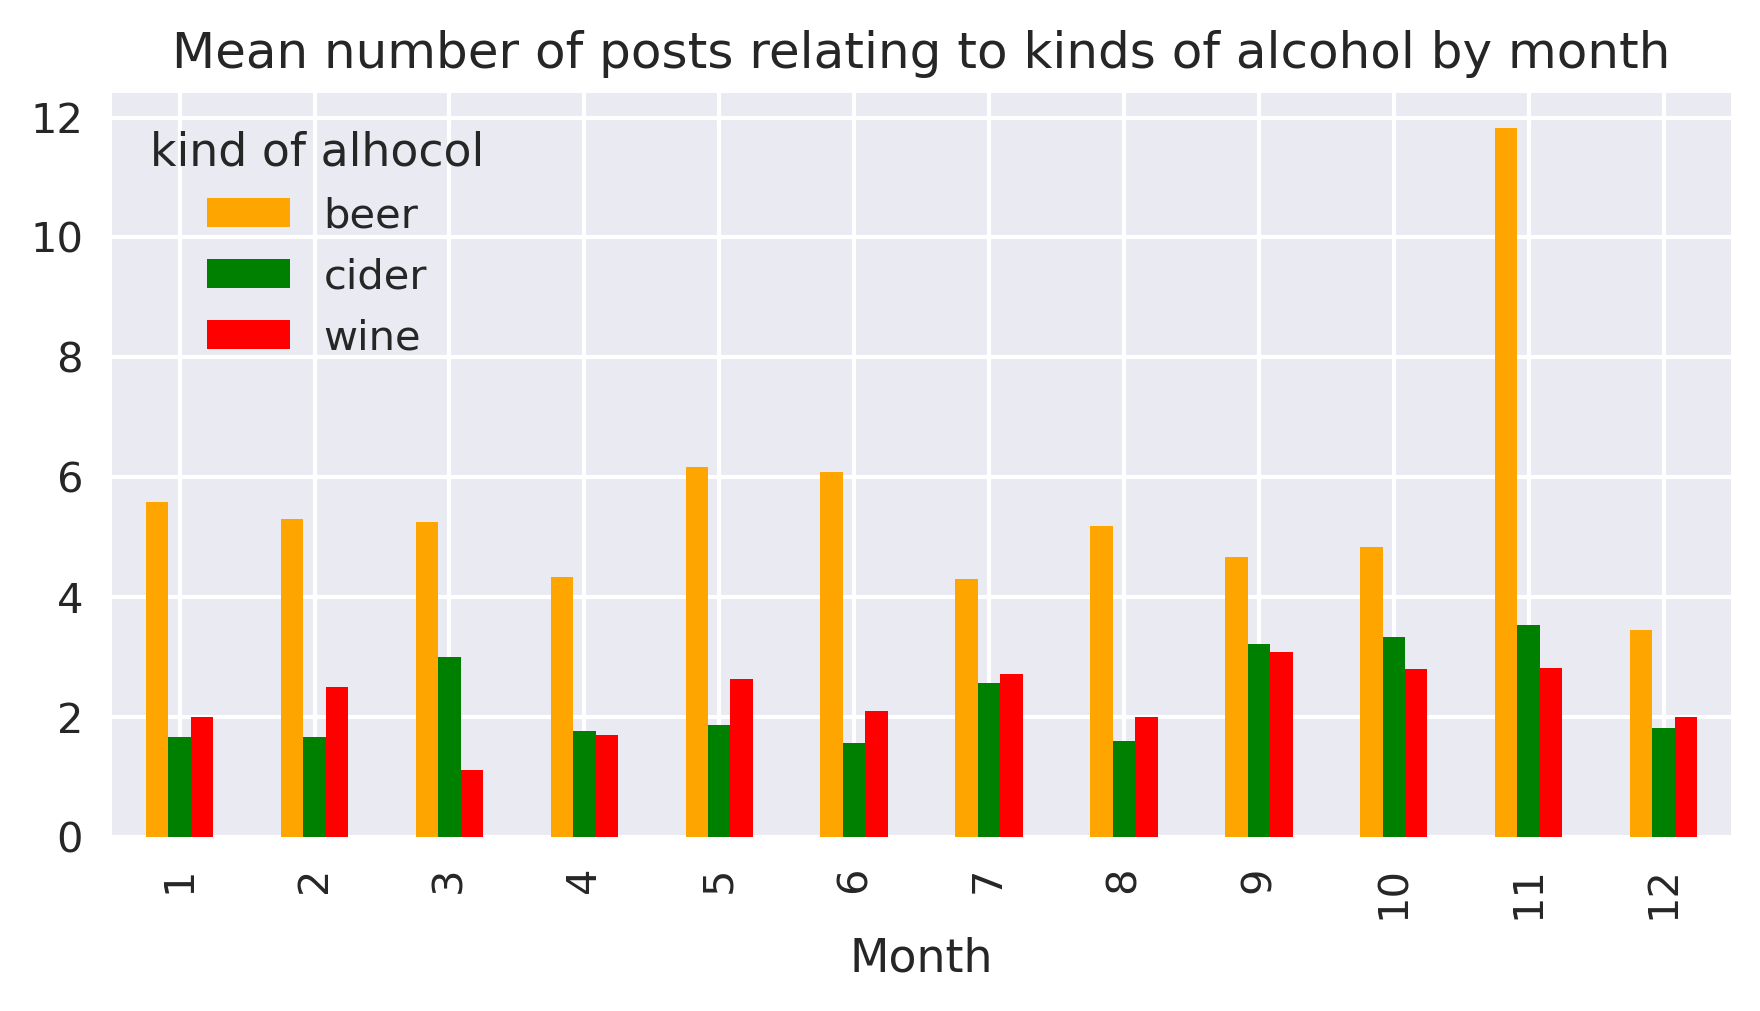
\includegraphics[width=0.7\textwidth]{homebrewing/h1.png}
        \caption*{Średnia ilość postów dotyczących badanych rodzajów alkoholu na miesiąc ogółem}
    \end{figure}
    \small Zależność została zbadana poprzez wyliczenie średniej ilości postów zawierających odpowiednie tagi (\it{beer}, \it{wine}, \it{cider}) na dany miesiąc w roku.
\end{frame}

\begin{frame}{Porównanie popularności pytań o piwo, wino i cydr}
    \begin{figure}[t]
        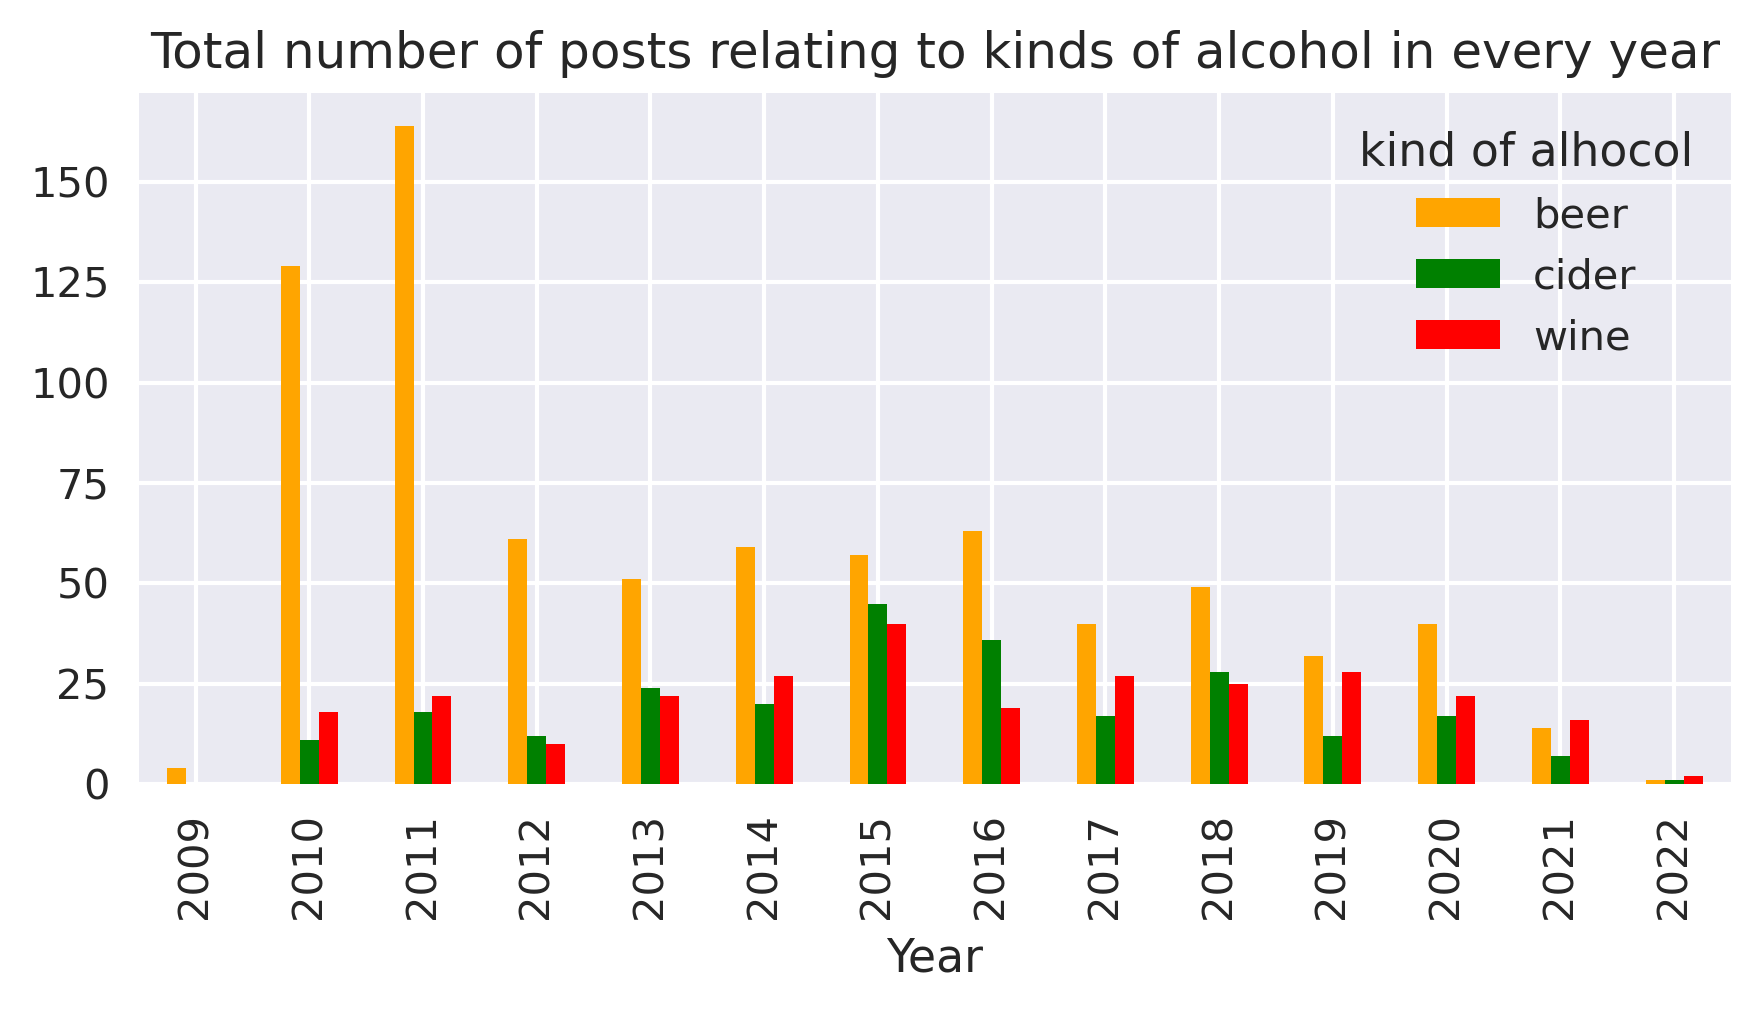
\includegraphics[width=0.7\textwidth]{homebrewing/h2.png}
        \caption*{Ilość postów dotyczących badanych rodzajów alkoholu w danym roku}
    \end{figure}
    \small Zależność została zbadana poprzez wyliczenie ilości postów zawierających odpowiednie tagi (\it{beer}, \it{wine}, \it{cider}) w danym roku.
\end{frame}

\begin{frame}{Prześledzenie popularności forum w czasie}
    \begin{figure}[t]
        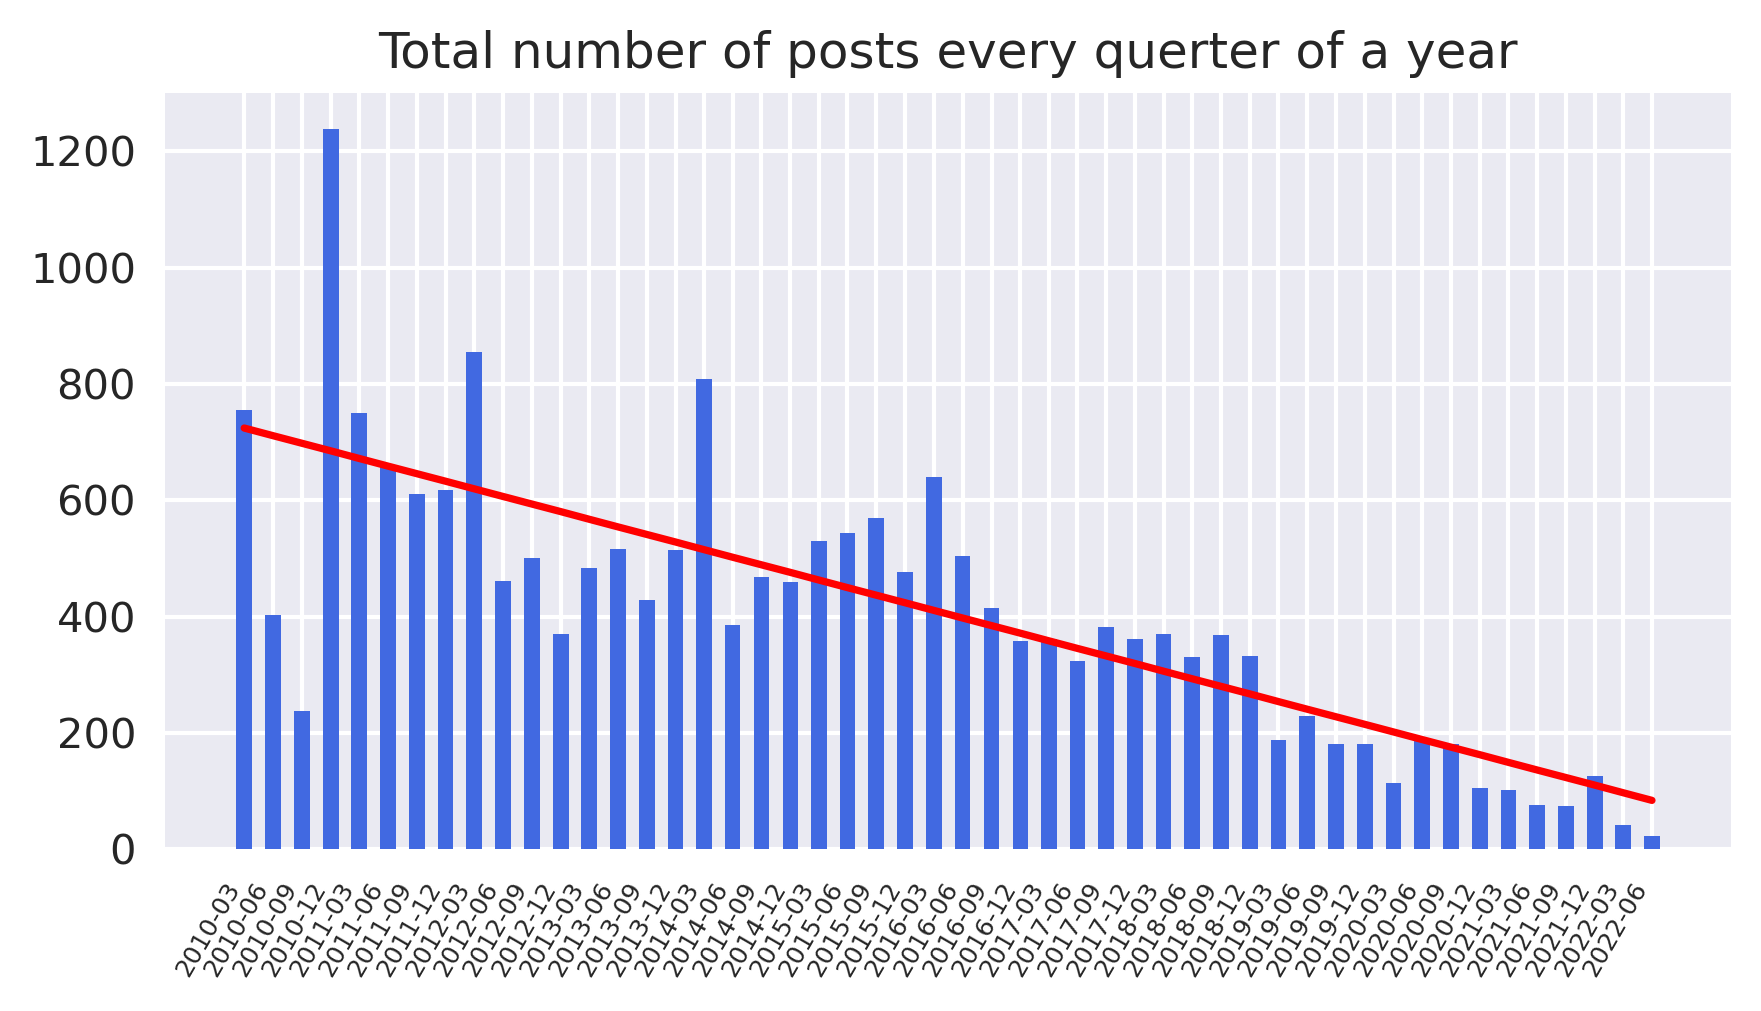
\includegraphics[width=0.7\textwidth]{homebrewing/h3.png}
        \caption*{Ilość postów ogółem w danym kwartale}
    \end{figure}
    \small Zależność została zbadana poprzez wyliczenie ilości postów w danym kwartale. Dopasowana została do tego linia trendu.
\end{frame}

\begin{frame}{Wnioski}
    \begin{enumerate}
        \item Pytania ,,piwne'' pojawiają się dużo częściej niż te dotyczące cydru czy wina.
        \item Znacząca średnia ilość pytań ,,piwnych'' w listopadzie.
        \item Znacząca ilość pytań ,,piwnych'' w latach 2010 i 2011.
        \item Znaczący wzrost postów ogółem w czwartym kwartale roku 2010 - prawdopodobnie odpowiada za skoki zaobserwowane wcześniej.
        \item Ogólny spadek ilości nowych postów - wymieranie forum.
    \end{enumerate}
\end{frame}

\begin{frame}{Badanie najbardziej intensywnego okresu w życiu forum}
    \begin{figure}[t]
        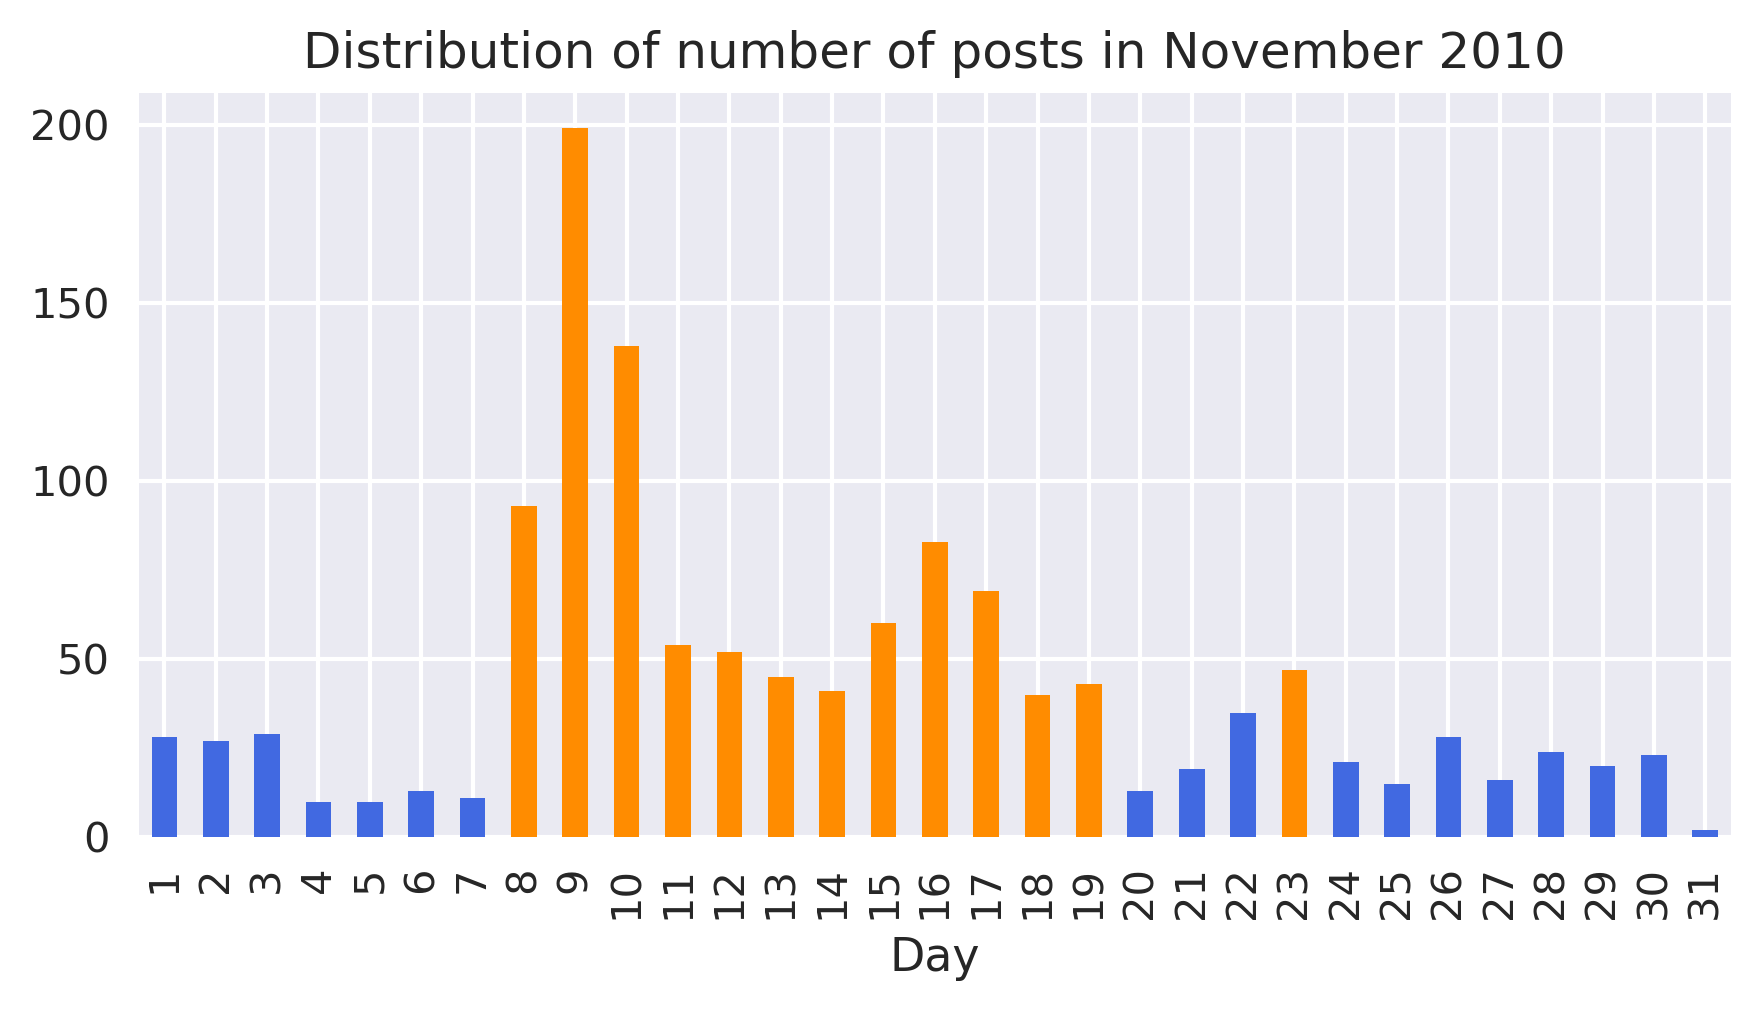
\includegraphics[width=0.7\textwidth]{homebrewing/h4.png}
        \caption*{Rozkład ilości postów w listopadzie 2010}
    \end{figure}
    \small Wyliczenie ilości postów w danym dniu w tym okresie. Pomarańczowe słupki oznaczają przekroczenie 40-stu postów.
\end{frame}

\begin{frame}{Badanie najbardziej intensywnego okresu w życiu forum}
    Dalej badane będzie 10 dni począwszy od 8 listopada 2010 w porównaniu z danymi z całego życia forum. Porównanie między tymi zbiorami będą badane z uwagi na diametralną różnicę w ilości postów publikowanych przez dni następujące po 8 listopada 2010.
\end{frame}

\begin{frame}{Badanie najbardziej intensywnego okresu w życiu forum}
    \begin{figure}[t]
        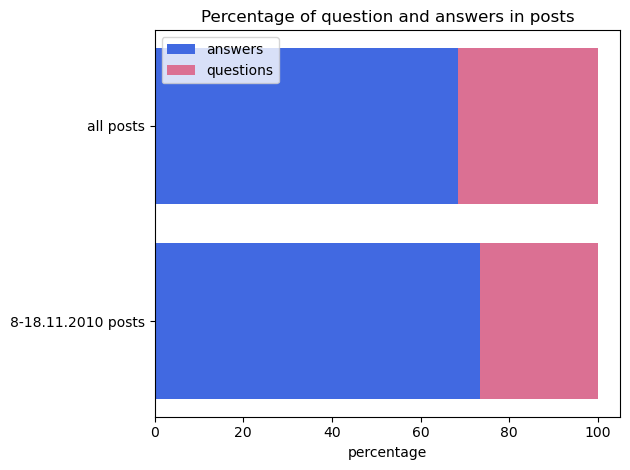
\includegraphics[width=0.6\textwidth]{homebrewing/h5.png}
        \caption*{Porównanie ilości pytań i odpowiedzi w postach (procentowo)}
    \end{figure}
    \small Zależność została zbadana grupując zbiory postów z danych okresów na pytania i odpowiedzi.
\end{frame}



\begin{frame}{Badanie najbardziej intensywnego okresu w życiu forum}
    \begin{figure}[t]
        \centering
        \subfloat{{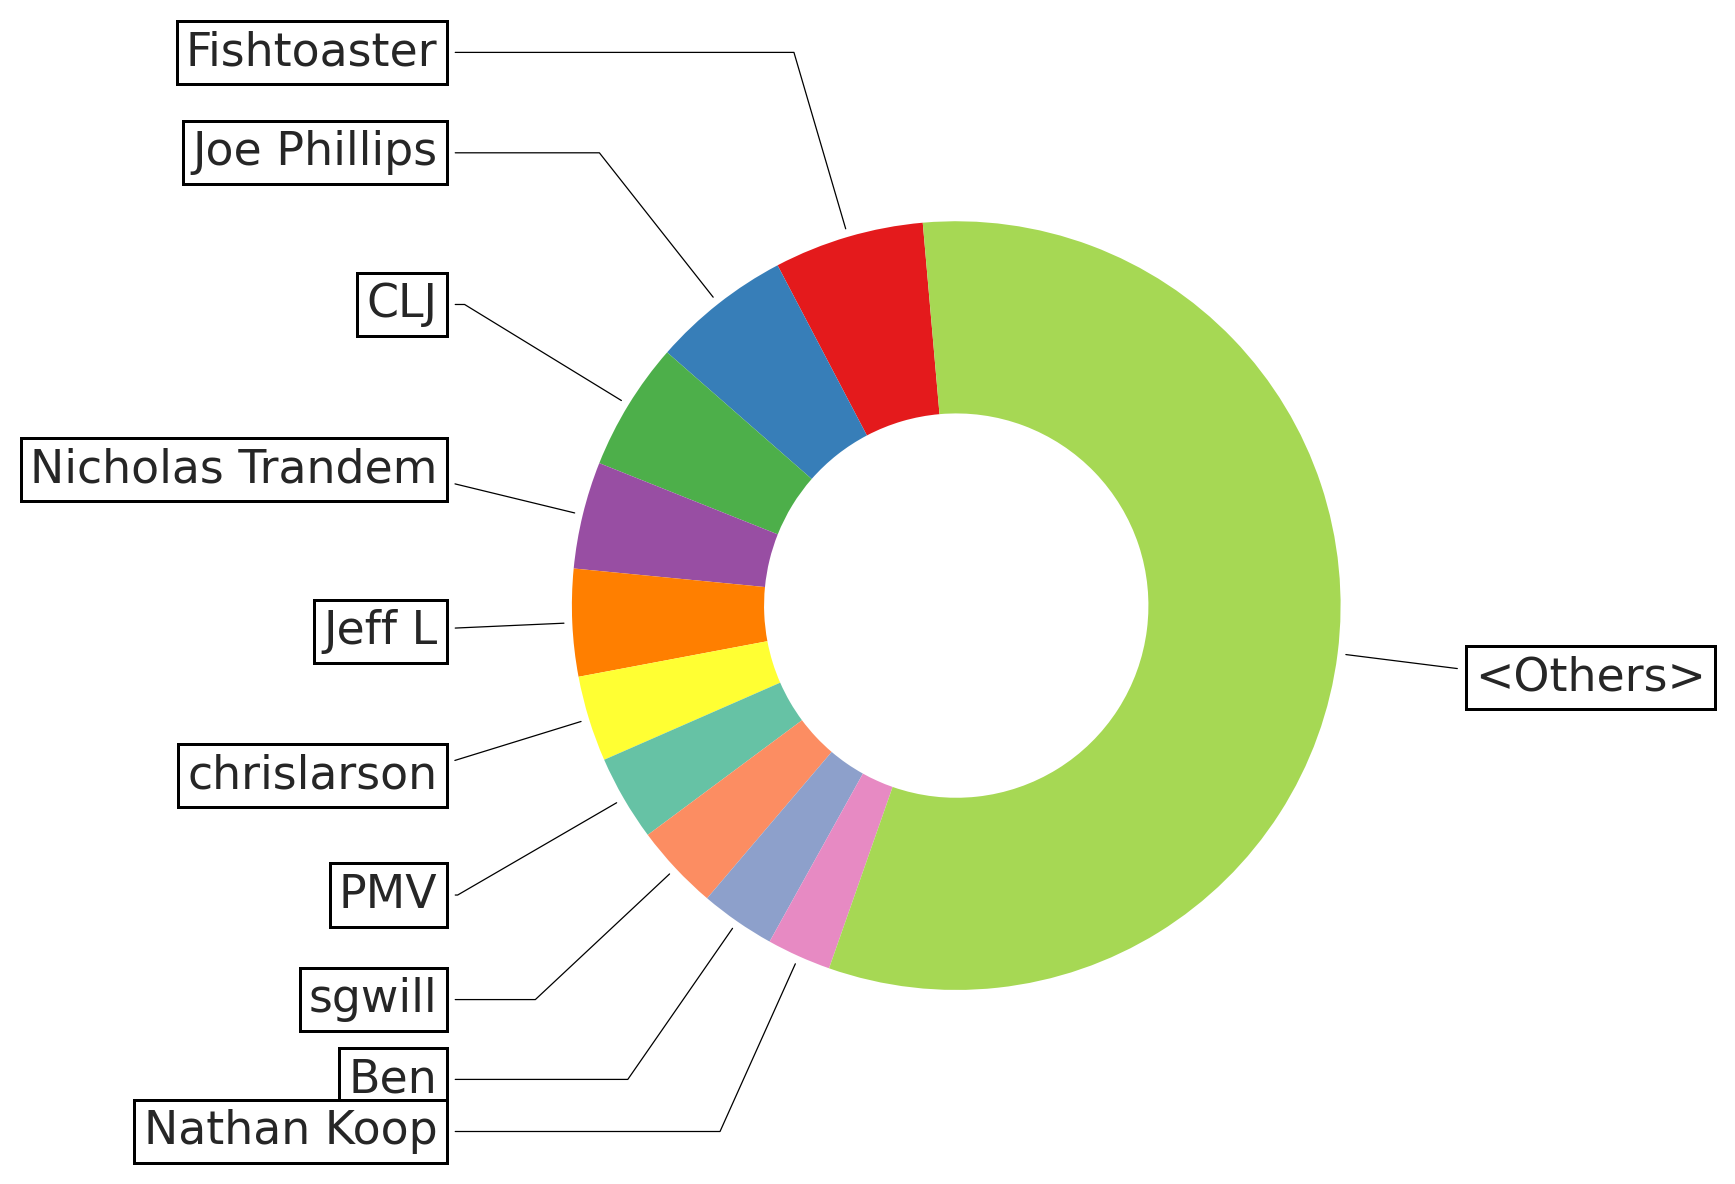
\includegraphics[width=0.45\textwidth]{homebrewing/h6_q_nov.png} }}%
        \qquad
        \subfloat{{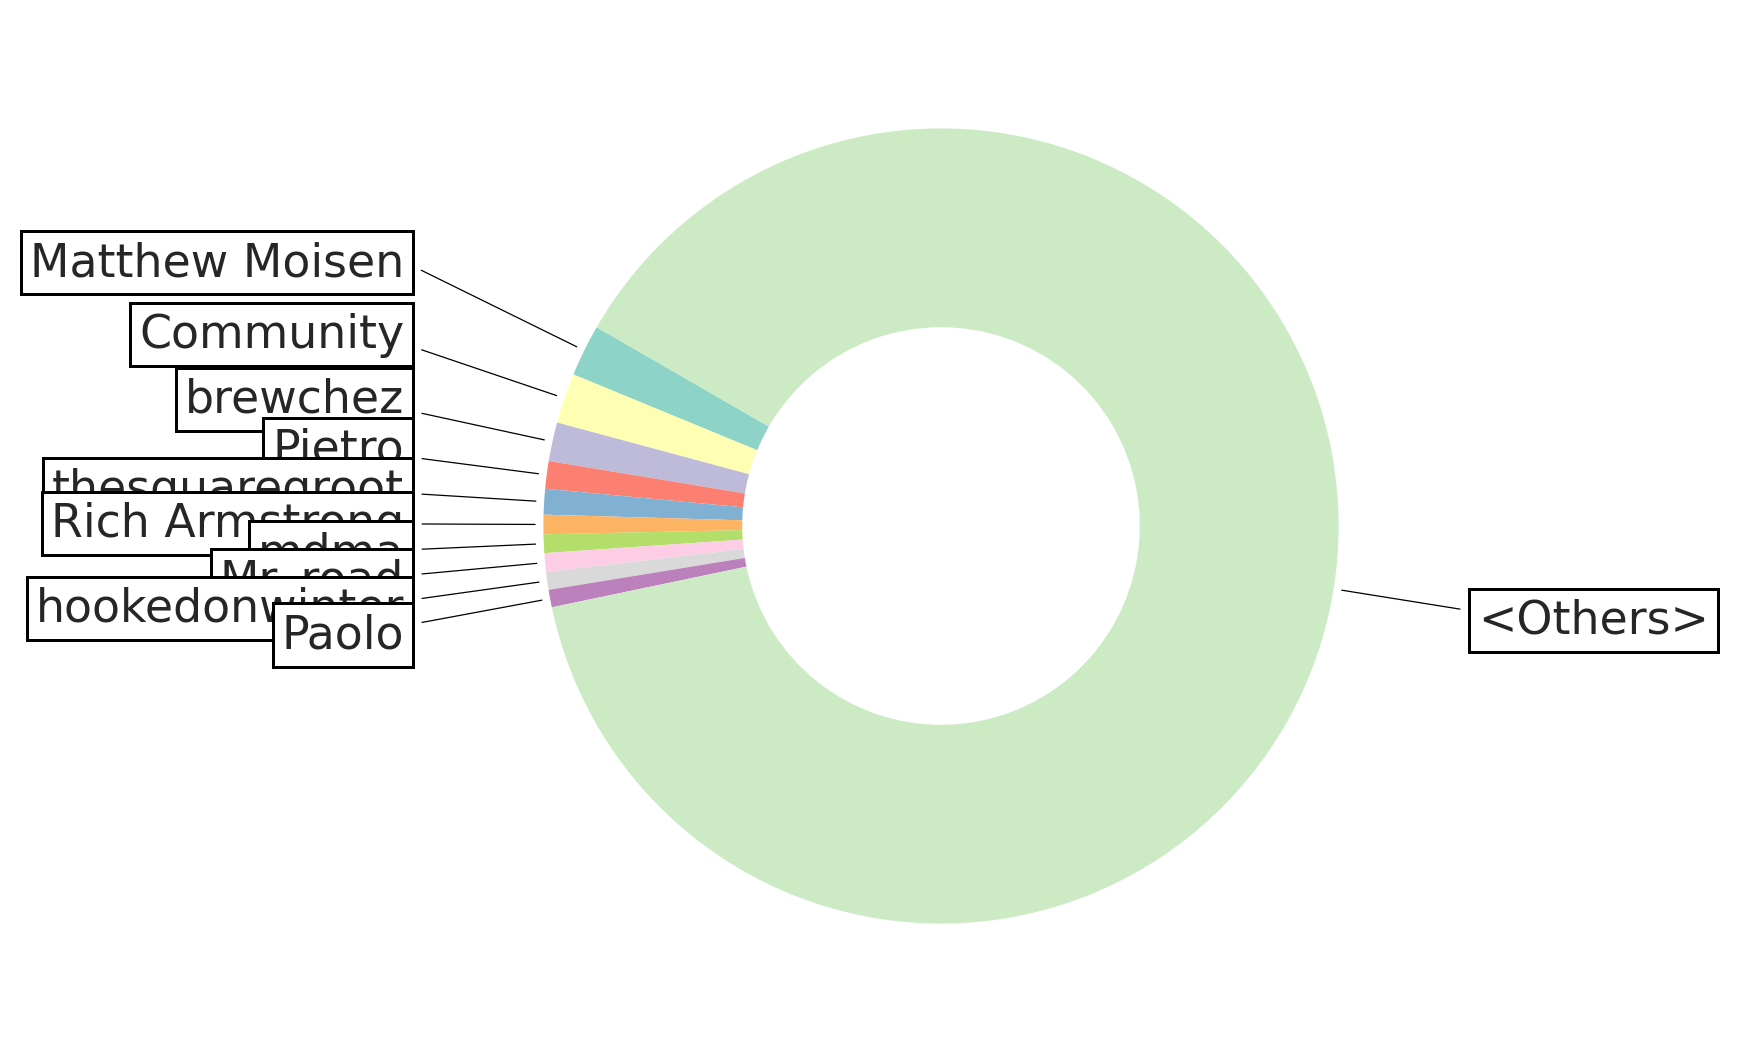
\includegraphics[width=0.45\textwidth]{homebrewing/h6_q_all.png} }}%
        \caption*{Porównanie jak dużą część pytań zadało top10 najbardziej aktywnych autorów pytań (po lewej okres 8-18.11.2010, po prawej całe forum).}
        \label{fig:example}%
    \end{figure}
    \small Zależność została zbadana grupując posty według nazw autorów (z tabeli użytkowników).
\end{frame}

\begin{frame}{Badanie najbardziej intensywnego okresu w życiu forum}
    \begin{figure}[t]
        \centering
        \subfloat{{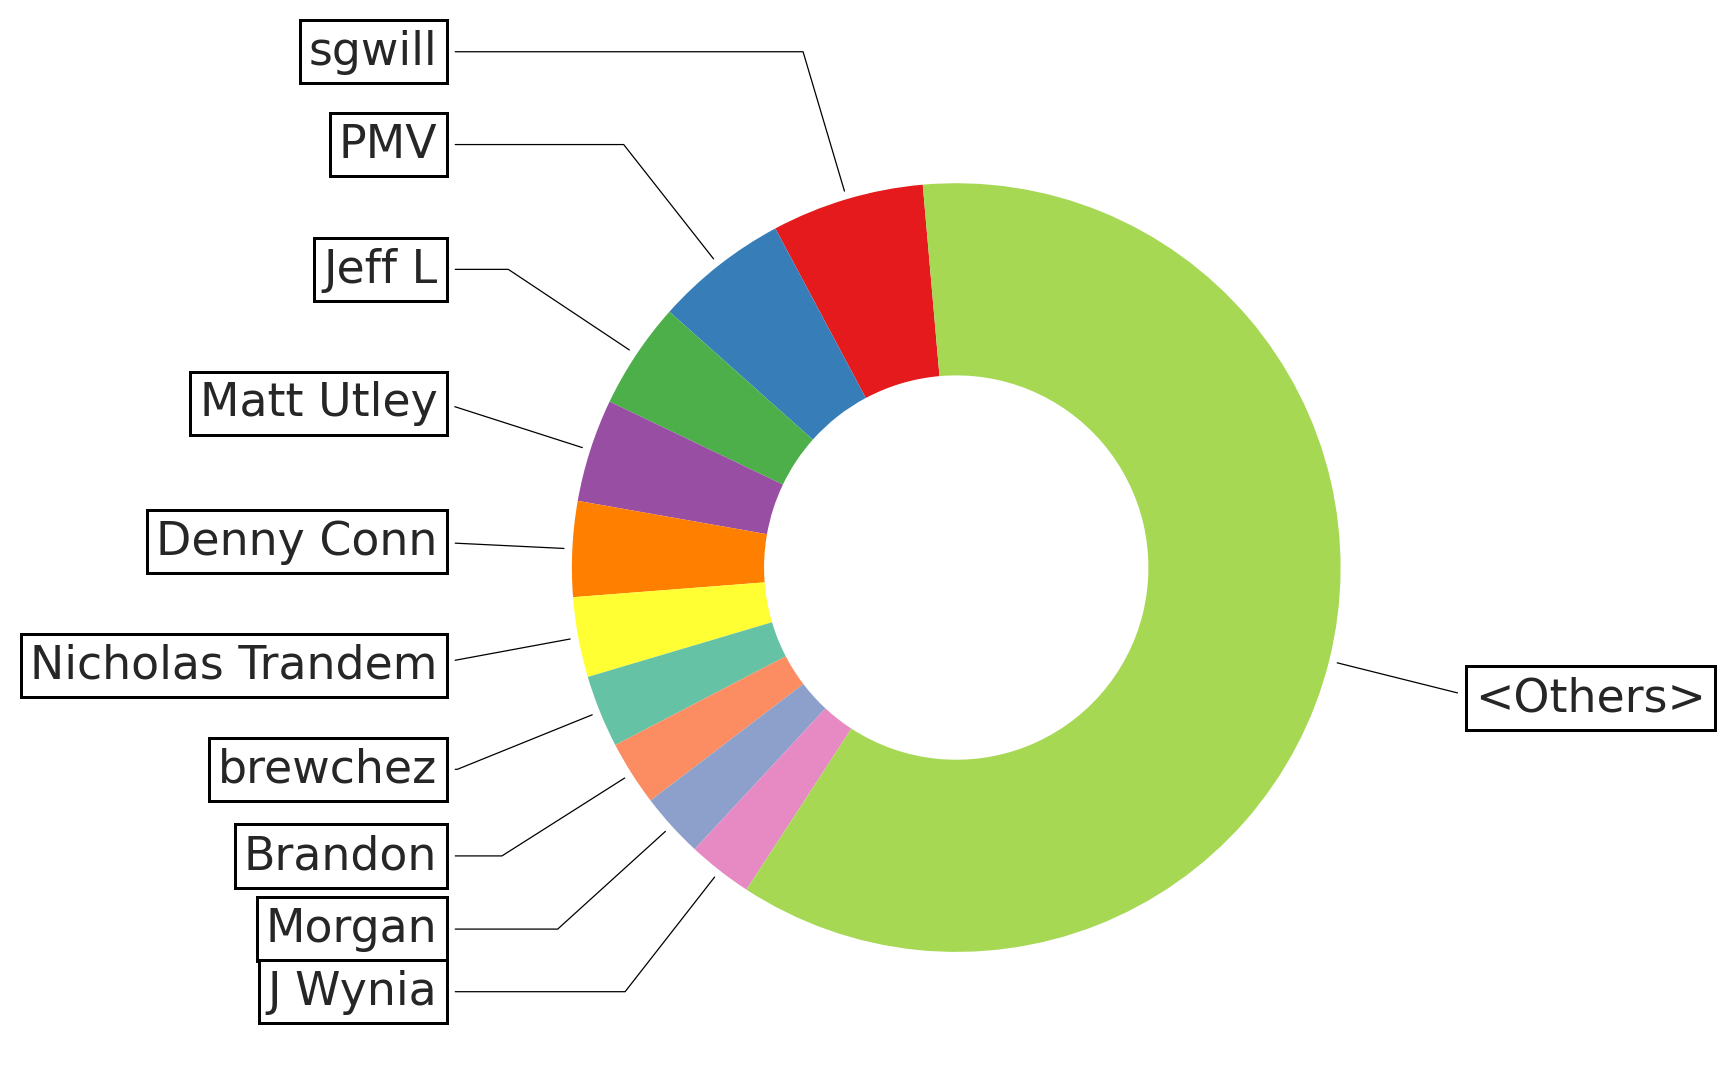
\includegraphics[width=0.45\textwidth]{homebrewing/h6_a_nov.png} }}%
        \qquad
        \subfloat{{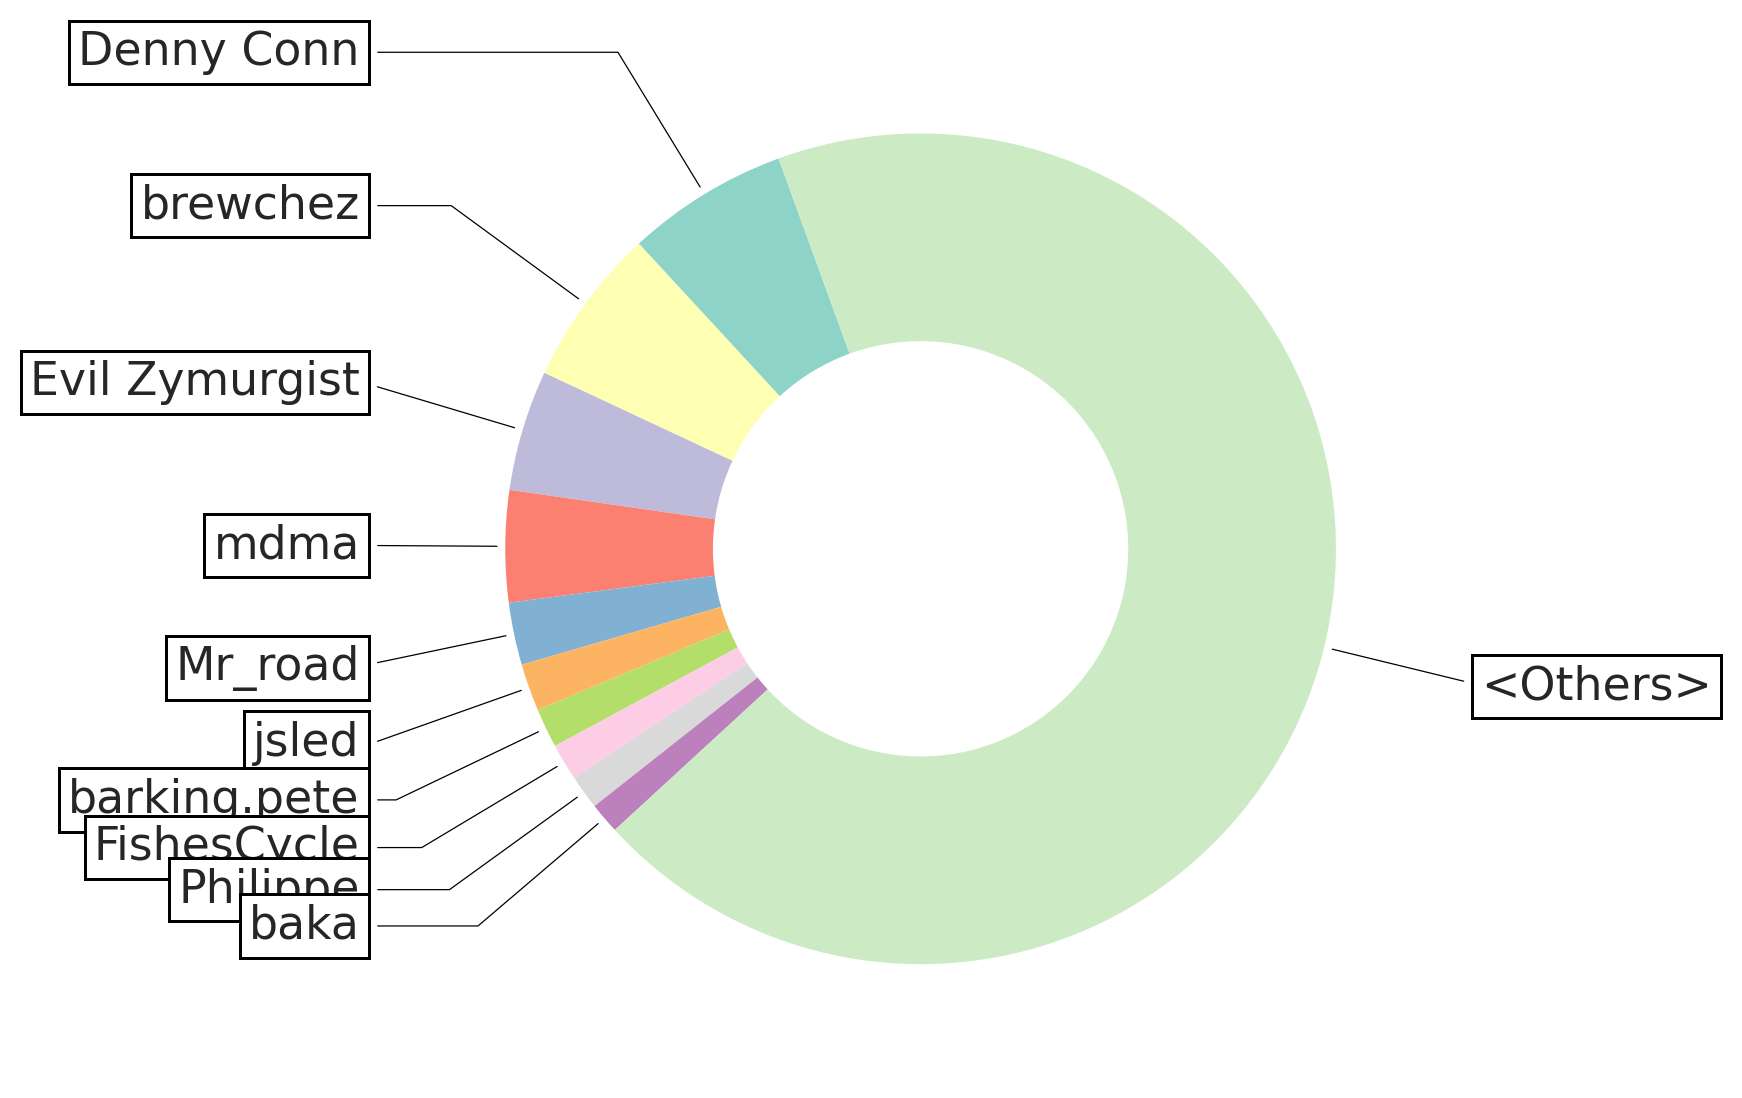
\includegraphics[width=0.45\textwidth]{homebrewing/h6_a_all.png} }}%
        \caption*{Porównanie jak dużą część odpowiedzi udzieliło top10 najbardziej aktywnych autorów odpowiedzi (po lewej okres 8-18.11.2010, po prawej całe forum).}
        \label{fig:example}%
    \end{figure}
    \small Zależność została zbadana grupując posty według nazw autorów (z tabeli użytkowników).
\end{frame}

\begin{frame}{Wnioski końcowe}
    \begin{enumerate}
        \item W intensywnym okresie nie zadano większej ilości pytań
        \item Za to najbardziej aktywni autorzy pytań zadali ich w intensywnym okresie dużo więcej niż dzieje się to średnio.
        \item Nie można stwierdzić podobnej zależności dla autorów odpowiedzi. Grono ekspertów przejawiało podobną aktywność w obu okresach.
        \item Najaktywniejszy ogólnie ekspert jest czwartym najaktywniejszym ekspertem z intensywnego okresu.
    \end{enumerate}
\end{frame}


\begin{frame}{Badanie najbardziej intensywnego okresu w życiu forum}
   \begin{figure}[t]
        
\includegraphics[width=\textwidth]{homebrewing/meta.png}
        \caption*{Wyjaśnienie nagłego wzrostu aktywności w roku 2010 z metaforum}
    \end{figure}
\end{frame}


\end{document}